\chapter{ICMP}
ICMP (Internet Control Message protocol) messages are embedded into IP datagrams\cite{RFC792}. ICMP can also be seen as a protocol that makes use of IP.
\begin{figure}[H]
\centering
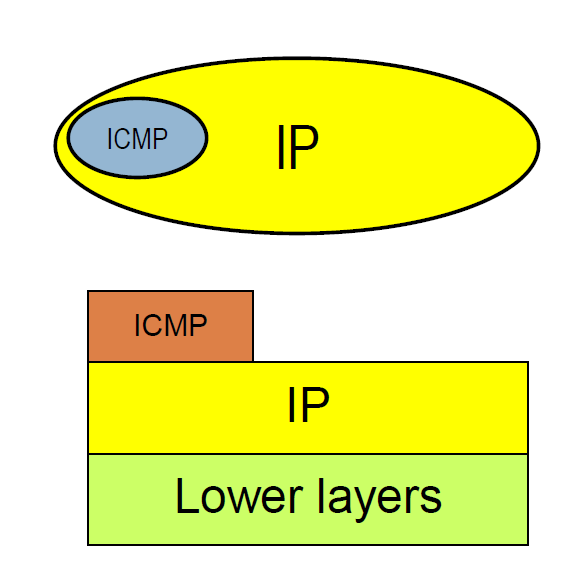
\includegraphics[scale=0.35, angle=0]{./Images/ICMP/ICMP_embedding}
\caption{\footnotesize{How ICMP is embedded in IP datagrams.}}
\end{figure}

The main controls, made by ICMP, are: 
\begin{itemize}
\item{\textbf{Error management (passive)}
\begin{itemize}
\item{Destination unreachable}
\item{Time expired (TTL or fragment reassembly timer)}
\item{Data inconsistency}
\item{Flow control}
\end{itemize}
}
\item{\textbf{Active mode}\\
Echo + Echo Reply (ping Unix)
}\\
\end{itemize}
In the IP header, the field protocol takes value 1 and indicates that the payload is an ICMP message.
\begin{figure}[H]
\centering
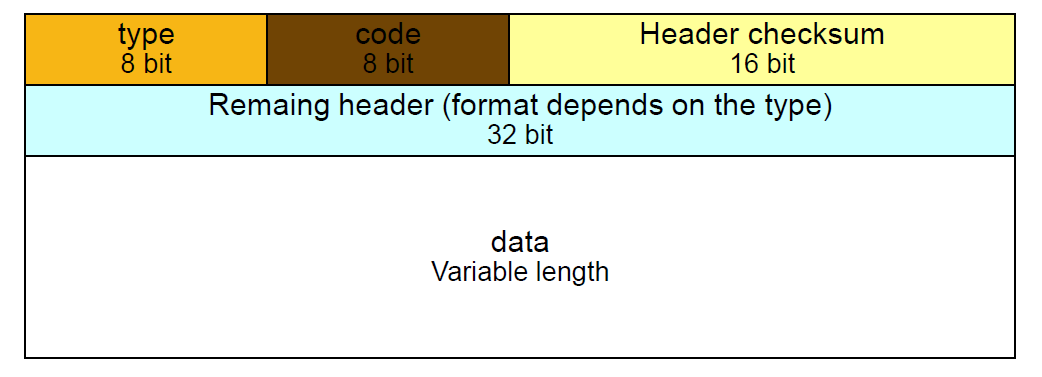
\includegraphics[scale=0.35, angle=0]{./Images/ICMP/ICMP_message_format}
\caption{\footnotesize{Format of ICMP message.}}
\end{figure}
\begin{table}[H]
\centering \footnotesize
\begin{tabular}{|l|l|}
\hline
0 & {Echo reply}\\
\hline
3 & {Destination unreachable}\\
\hline
4 & {Source Quench}\\
\hline
5 & {Redirect (change a route)}\\
\hline
8 & {Echo request}\\
\hline
11 & {Time exceeded}\\
\hline
12 & {Parameter problem}\\
\hline
13 & {Timestamp request}\\
\hline
14 & {Timestamp reply}\\
\hline
17 & {Address mask request}\\
\hline
18 & {Address mask reply}\\
\hline
\end{tabular}
\caption{Type values.}
\end{table}
Other header fields depend on the type of message that must to be generated.
\section{Main rules of ICMP error messages}
\begin{itemize}
\item{No ICMP error message will be generated in response to a datagram carrying an ICMP error message}
\item{No ICMP error message will be generated for a fragmented datagram that is not the first fragment}
\item{No ICMP error message will be generated for a datagram having a multicast address}
\item{No ICMP error message will be generated for a datagram having a special address such as 127.0.0.0 or 0.0.0.0.}
\end{itemize}
\textbf{NOTE:} \textit{No all routers generate ICMP messages.}

\section{Types of ICMP messages}
\subsection{Echo}
Echo-request and Echo-reply are used to check the reachability of hosts and routers.\\
Upon receiving an Echo-request, the ICMP entity of a device immediately replies with Echo reply.
\begin{figure}[H]
\centering
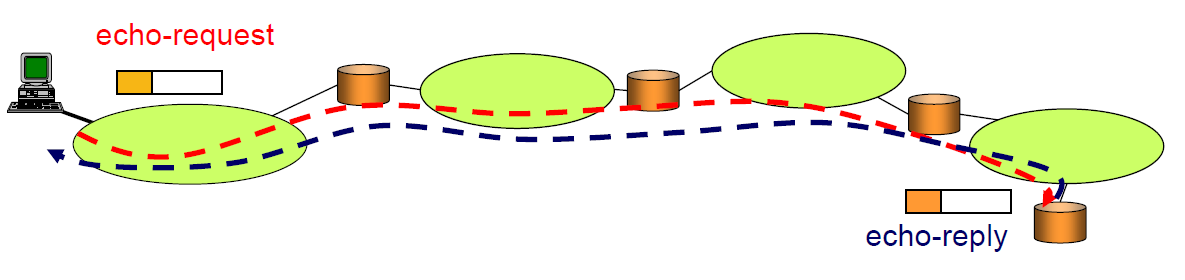
\includegraphics[scale=0.35, angle=0]{./Images/ICMP/ECHO_working}
\caption{\footnotesize{ECHO requests and replies in practice.}}
\end{figure}
\begin{table}[H]
\centering \footnotesize
\begin{tabular}{c|l}
\multirow{2}{*}{Type:} & {$\Rightarrow 8$ request}\\
& {$\Rightarrow 0$ reply}\\
\end{tabular}
\end{table}
\begin{center}
Code: $\Rightarrow 0$\\
\end{center}
\begin{figure}[H]
\centering
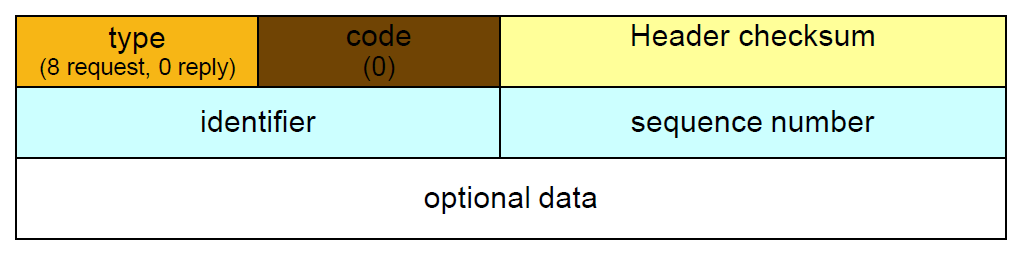
\includegraphics[scale=0.35, angle=0]{./Images/ICMP/ECHO_format}
\caption{\footnotesize{Format of ECHO message.}}
\end{figure}
Other important fields of Echo messages are:
\begin{itemize}
\item{\textbf{Identifier}\\
Each \textbf{Echo} message has an identifier, defined in the \textbf{Echo request}, and replicated in the \textbf{Echo reply}.
}
\item{\textbf{Sequence number}\\
Consecutive requests may have the same identifier and change from others for sequence number only. The sequence number is used to measure the RTT and count the number of lost bytes.
}
\item{\textbf{Optional data}\\
The sender can add \textbf{Optional data} to the request message. The data will be replicated in the reply message.
}
\end{itemize}
The payload of Echo (IP datagram) is used to check the capacity of a link (RTT is bigger if the link has small bitrate).

\subsection{Destination unreachable}
When a packet is dropped, an error message is returned, through ICMP, to the source.
\begin{center}
Type: $\Rightarrow 3$\\
\end{center}
\begin{figure}[H]
\centering
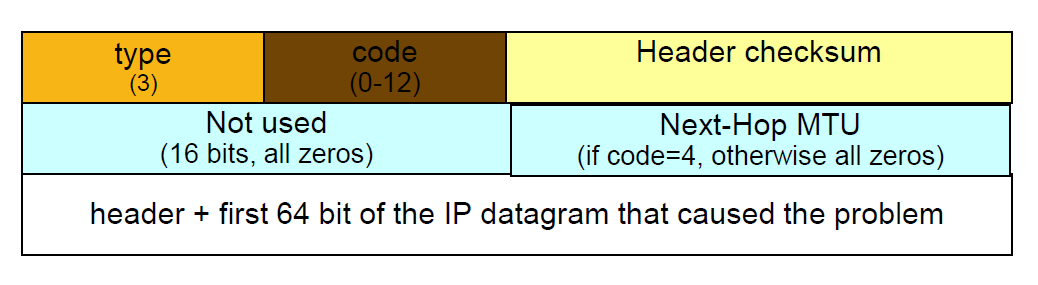
\includegraphics[scale=0.35, angle=0]{./Images/ICMP/Destination_unreachable}
\caption{\footnotesize{Destination unreachable message format.}}
\end{figure}
The “code” field of the ICMP message refers to the type of error that has generated the message. 
\begin{table}[H]
\centering \footnotesize
\begin{tabular}{|l|l|l|}
\multicolumn{1}{c}{Code} & \multicolumn{1}{c}{Description} & \multicolumn{1}{c}{References}\\
\hline
\footnotesize{0} & {\footnotesize{Network unreachable error.}} & {\footnotesize{RFC 792}}\\
\hline
\footnotesize{1} & {\footnotesize{Host unreachable error.}} & {\footnotesize{RFC 792}}\\
\hline
\multirow{2}{*}{\footnotesize{2}} &	{\footnotesize{Protocol unreachable error.}} & \multirow{2}{*}{\footnotesize{RFC 792}}\\
& {\footnotesize{Sent when the designated transport protocol is not supported.}} &	\\
\hline
\multirow{3}{*}{\footnotesize{3}} & {\footnotesize{Port unreachable error.}} & \multirow{3}{*}{\footnotesize{RFC 792}}\\
& {\footnotesize{Sent when the designated transport protocol is unable to demultiplex}} &\\
& {\footnotesize{the datagram but has no protocol mechanism to inform the sender.}} &\\
\hline
\multirow{2}{*}{\footnotesize{4}} & {\footnotesize{The datagram is too big.}} & \multirow{2}{*}{\footnotesize{RFC 792}}\\
& {\footnotesize{Packet fragmentation is required but the DF bit in the IP header is set.}} &\\
\hline
\footnotesize{5} & {\footnotesize{Source route failed error.}} & {\footnotesize{RFC 792}}\\
\hline
\footnotesize{6} & {\footnotesize{Destination network unknown error.}} & {\footnotesize{RFC 1122}}\\
\hline
\footnotesize{7} & {\footnotesize{Destination host unknown error.}} & {\footnotesize{RFC 1122}}\\
\hline
\footnotesize{8} & {\footnotesize{Source host isolated error. (Obsolete)}} & {\footnotesize{RFC 1122}}\\
\hline
\footnotesize{9} & {\footnotesize{The destination network is administratively prohibited.}} & {\footnotesize{RFC 1122}}\\
\hline
\footnotesize{10} & {\footnotesize{The destination host is administratively prohibited.}} & {\footnotesize{RFC 1122}}\\
\hline
\footnotesize{11} & {\footnotesize{The network is unreachable for Type Of Service.}} & {\footnotesize{RFC 1122}}\\
\hline
\footnotesize{12} & {\footnotesize{The host is unreachable for Type Of Service.}} & {\footnotesize{RFC 1122}}\\
\hline
\multirow{2}{*}{\footnotesize{13}} & {\footnotesize{Communication Administratively Prohibited.}} & \multirow{2}{*}{\footnotesize{RFC 1812}}\\
& {\footnotesize{Administrative filtering prevents a packet from being forwarded.}} & 	\\
\hline
\multirow{3}{*}{\footnotesize{14}} & {\footnotesize{Host precedence violation.}} & \multirow{2}{*}{\footnotesize{RFC 1812}}\\
& {\footnotesize{The requested precedence is not permitted for the particular combination}} &\\
& {\footnotesize{of host or network and port.}} & \\
\hline
\multirow{2}{*}{\footnotesize{15}} & {\footnotesize{Precedence cutoff in effect.}} & 	{\footnotesize{RFC 1812}}\\
& {\footnotesize{The precedence of datagram is below the level set by the network administrators.}} &\\
\hline
\end{tabular}
\caption{\footnotesize{Code values.}}
\end{table}
\subsection{Time exceeded}
It's generated when some packets are missing or don't reach the destination.
\begin{center}
Type: $\Rightarrow 3$\\
\end{center}
\begin{figure}[H]
\centering
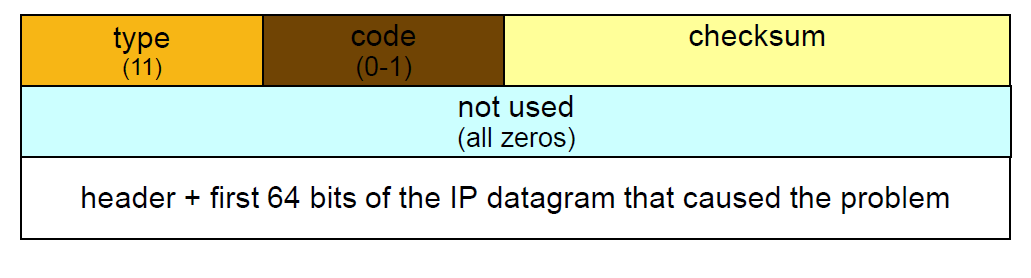
\includegraphics[scale=0.35, angle=0]{./Images/ICMP/Time_exceeded}
\caption{\footnotesize{Time exceeded message format.}}
\end{figure}
The main problems, that generate this message, are: 
\begin{table}[H]
\centering\footnotesize
\begin{tabular}{|c|l|}
\multicolumn{1}{c}{\textbf{Code}} & \multicolumn{1}{c}{\textbf{Problem}}\\
\hline
\multirow{2}{*}{0} & {Generated by a router when it decreases the TTL to 0}\\
\cline{2-2}
{ } & {Returned to the source of the IP datagram}\\
\hline
\multirow{2}{*}{1} & {Generated by the destination, when some fragments are}\\
{} & {missing, after the fragment reasembly timer expires}\\
\hline
\end{tabular}
\end{table}

\subsection{Parameter problem}
It's generated when there are some wrong formats or unknown options. 
\begin{center}
Type: $\Rightarrow 12$\\
\end{center}
\begin{figure}[H]
\centering
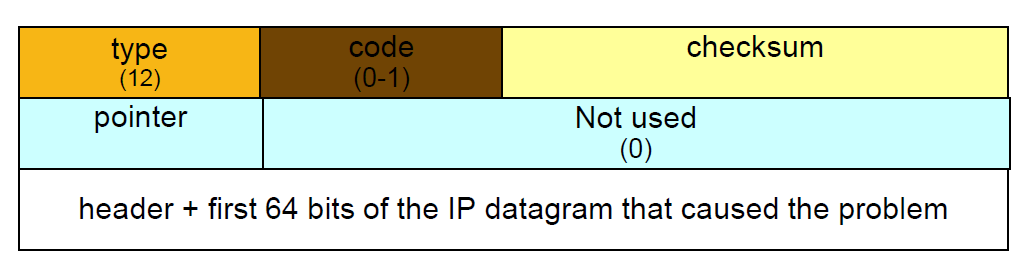
\includegraphics[scale=0.35, angle=0]{./Images/ICMP/Parameter_problem}
\caption{\footnotesize{Format of Parameter problem message.}}
\end{figure}
The main problems generated by this message are:
\begin{table}[H]
\centering \footnotesize
\begin{tabular}{|c|l|}
\multicolumn{1}{c}{\textbf{Code}} & \multicolumn{1}{c}{\textbf{Problem}}\\
\hline
\multirow{2}{*}{0} & {If the header of an IP datagram contains a malformed}\\
{}& {field (violate format)}\\
\hline
\multirow{2}{*}{1} & {Used when an option is unknown or a certain operation}\\
{}& {cannot be carried out}\\
\hline
\end{tabular}
\end{table}
\subsection{Redirect}
It's generated by a router to require the source to use a different router
\begin{center}
Type: $\Rightarrow 5$\\
Code: $\Rightarrow 0-3$\\
\end{center}
\begin{figure}[H]
\centering
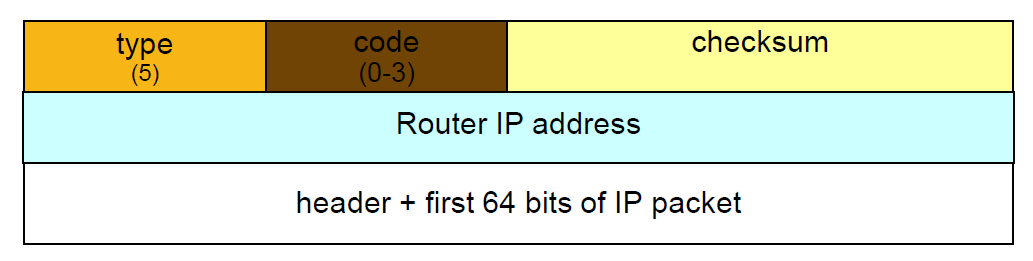
\includegraphics[scale=0.35, angle=0]{./Images/ICMP/Redirect}
\caption{\footnotesize{Format of Redirect message.}}
\end{figure}

\begin{figure}[H]
\centering
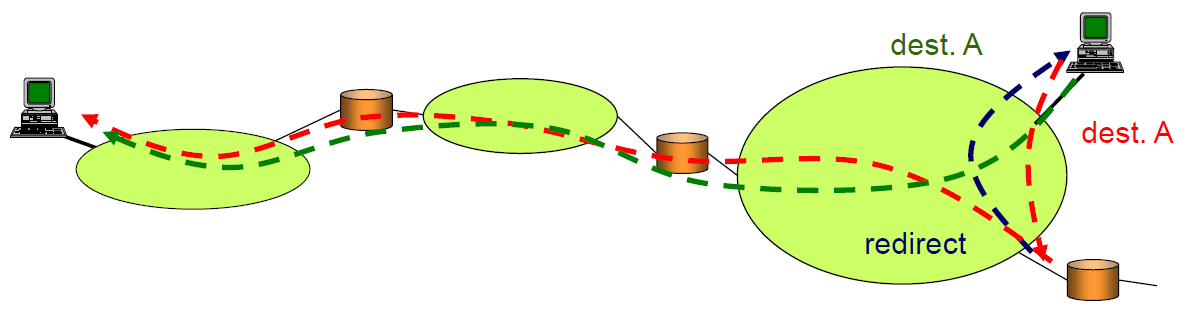
\includegraphics[scale=0.35, angle=0]{./Images/ICMP/Redirect_use}
\caption{\footnotesize{How Redirect messages are used.}}
\end{figure}

\subsection{Timestamp request e reply}
It's used to exchange clock information between source and destination.
\begin{table}[H]
\centering \footnotesize
\begin{tabular}{c|l}
\multirow{2}{*}{Type:} & {$\Rightarrow 13$ request}\\
& {$\Rightarrow 14$ reply}\\
\end{tabular}
\end{table}

\begin{center}
Code: $\Rightarrow 0$\\
\end{center}
\begin{figure}[H]
\centering
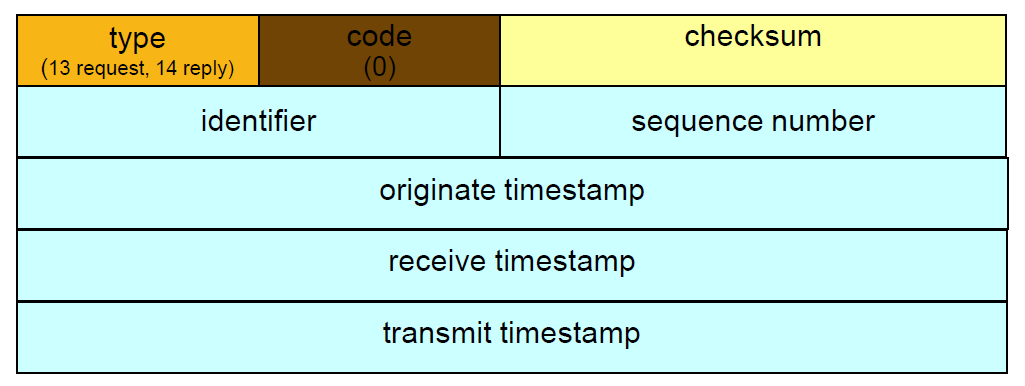
\includegraphics[scale=0.35, angle=0]{./Images/ICMP/Timestamp}
\caption{\footnotesize{Format of Timestamp request and reply.}}
\end{figure}
\begin{itemize}
\item{\textbf{Originate timestamp}\\
inserted by the source
}
\item{\textbf{Receive timestamp}\\
inserted by the destination right after receiving the ICMP message
}
\item{\textbf{Transmit timestamp}\\
inserted by the destination just before returning the ICMP message
}
\end{itemize}
\subsection{Address mask request and reply}
It's used to ask for the netmask of a router/host.
\begin{table}[H]
\centering \footnotesize
\begin{tabular}{c|l}
\multirow{2}{*}{Type:} & {$\Rightarrow 17$ request}\\
& {$\Rightarrow 18$ reply}\\
\end{tabular}
\end{table}
\begin{center}
Code: $\Rightarrow 0$\\
\end{center}
\begin{figure}[H]
\centering
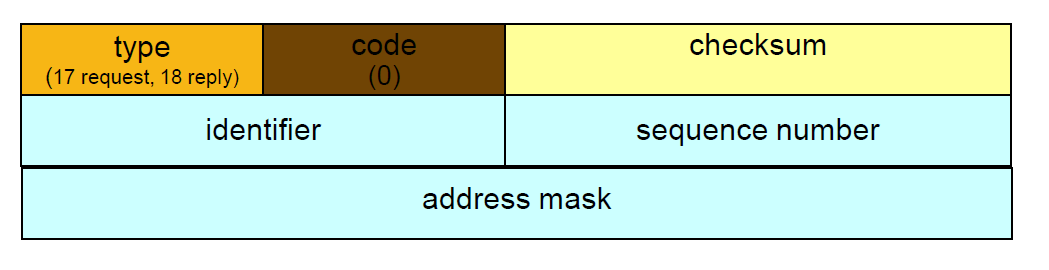
\includegraphics[scale=0.35, angle=0]{./Images/ICMP/Address_mask}
\caption{\footnotesize{Format of Address mask request and reply.}}
\end{figure}
\begin{itemize}
\item{\textbf{Address mask}\\
In the request message, it's void and it is populated by the device that replies to the request
}
\end{itemize}
